\graphicspath{{Images/}}

\section{The Basics of Quantum} \label{quantum_basics}
In its most general form, a quantum computer is a device that stores quantum particles in a controlled environment that is controlled in a such a way that these particles can be made to do what we want \cite{theunlockr}. QCs take advantage of fact that very small particles have unique rules and properties set out by quantum mechanics and quantum physics. In comparison with the properties of larger atoms, quantum particles seem as if they bend the rules of space and time. Acting in a seemingly random manner provable and made a little bit more predictable with mathematical properties and proofs, we use controlled environments with low temperatures, superconducting circuits, fiber optic cables, and more \cite{unc_qc} to control quantum particles like photons in such a way that allows us to do computations on them and use them to solve problems. Where classical computers use bits in distinct zero or one states to store information and use mathematical transformations to do computations and solve problems, quantum computers use quantum bits, referred to as \textbf{\glspl{qubit}}. Some defining properties of qubits that make quantum computers distinct from classical computers are explained below.  

    \subsection{Entanglement}
    The first unique property that quantum particles follow is that of entanglement. It is defined as thus: 
    \begin{quote}
        \textbf{\Gls{entanglement}} is where the quantum state of each particle within a set cannot be described independently of the state of the other particles even when the particles are separated by a large distance. It has been found that position, momentum, spin, and polarization can all be perfectly correlated \cite{entanglement}.
    \end{quote}

    If we imagine qubits as particles that spin, we can compare traditional bits of zeroes and ones to qubits in a spin down state (which correlates to a natural-state of zero) and a spin up state (where this change in energy corresponds to a state of one). Entanglement tells us that given two entangled qubits, if one is spin up, and the relation between them is that they are inverses of each other, the other will be spin down, and if one changes its spin direction the other will automatically change accord to their relation. Additionally, observational research has also shown that entangled qubits are "monogamous" \cite{info_is_quantum}, meaning the more entangled they are with each other, the less they will be with other qubits.
    
    \subsection{Superposition} \label{superposition}
    Imagining qubits in the directly opposing spin up and spin down states, opens the door to discuss in-between states. Schr\"{o}dinger's cat is a thought experiment by Edwin Schr\"{o}dinger introduced in 1935, and it is commonly referenced to explain the idea of superposition:
    
    \begin{quote}
        "A cat, a flask of poison, and a radioactive source are placed in a sealed box. If an internal radiation monitor (e.g. a Geiger counter) detects radioactivity (i.e. a single atom decaying), the flask is shattered releasing the poison which skills the cat. The Copenhagen interpretation [of quantum mechanics] implies that, after a while, the cat is simultaneously alive and dead. Yet, when one looks in the box, one sees the cat either alive or dead, but not both alive and dead." (See Figure \ref{fig:cat}) \cite{schrodinger}
    \end{quote}
    
    \begin{figure}[ht] 
        \centering
        \ffigbox[\FBwidth]
        {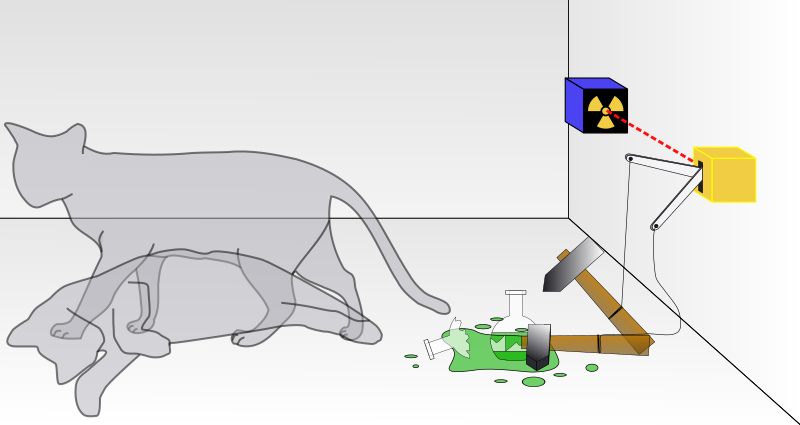
\includegraphics[width=0.65\textwidth]{Schrodingers_cat.png}}
        {
            \captionsetup{justification=centering}
            \caption{"Schr\"{o}dinger's cat: a cat, a flask of poison, and a radioactive source connected to a Geiger counter are placed in a sealed box. As illustrated, the objects are in a state of superposition: the cat is both alive and dead." \cite{schrodinger}}
            \label{fig:cat}
        }
    \end{figure}
    
    Originally intended as a criticism of how insensible the idea of superposition was, it went on to be used as a popular analogy for describing the exact principle it sought to criticize. It then went on to inspire further work that would build upon this premise. Charles Bennett explains the idea of superposition more directly:
    \begin{quote}
        "Between any two reliably distinguishable states in the physical system - not all states or pairs of states are reliably distinguishable - there are intermediate states that are not distinguishable from either one, and they correspond to intermediate directions in space, and the two states are reliably distinguishable if their directions are perpendicular. Any two perpendicular directions correspond to reliably distinguishable states, and any two directions that are not perpendicular correspond to a pair of states that are different but not reliably distinguishable." \cite{charles_b}
    \end{quote}

    Explained as simply as possible, superposition tells us that where a classical computer's bits must be a zero or one, qubits can be many things in between. Not only can it be more than two binary states, superposition tells us that in fact a qubit may be in all possible states at the same time. This increased complexity means that qubit states are often expressed using probabilities in something called \textbf{\gls{ket}} (sometimes referred to as Dirac notation). 

    \subsection{What this means}
    Superposition is the main property that makes quantum computers the ideal tool to evaluate high variable, high complexity problems especially when the problem involves trying to find the best solution from a series of possible sources (an example is the traveling salesman problem) because this property allows us to store and on some level track and represent collective states rather than singular binary states. The one caveat is that reading the state of a quantum system will destroy the superposition information. This is what makes quantum computers not very good at problems that require sorting, possibly performing worse than classical computers. 

    Entanglement is the main property that enabled, inspired, and currently supports the field of quantum communication and its research. It is has inspired schemes such as Bennett and Brassard's BB84 communication protocol, and the way that entangled particles reliably react across long distances has enabled communication schemes that utilize this property to have near instantaneous communication across very large distances.

    Beyond the basic properties of entanglement and superposition, there are a few more basic principles that limit quantum computers. The first property states that no quantum states can be cloned referred to as the no-cloning theorem. Secondly and somewhat relatedly, the exact polarization of a quantum particle or qubit or quantum state cannot be measured. Logically, being able to do one would enable the other and vice versa. These properties have posed issues when it comes to error checking and information transmission fidelity (i.e. what is sent is the same as what is received). Classical computers utilize many different schemes for error checking including parity bits, redundancy checks, and Hamming codes, and many of these involve some level of cloning. As it stands right now, quantum computers are still quite error prone due to the need to created adapted error checking schemes that don't rely on cloning. Multiple schemes have been suggested to combat this, but they have not yet been able to be implemented in a large scale way that would allow us to rigorously test their effectiveness \cite{shor}.








